\documentclass[12pt]{article}
\usepackage{style}
\usepackage{hyperref}
\usepackage{float}
\newcolumntype{L}[1]{>{\centering\let\newline\\\arraybackslash\hspace{0pt}}m{#1}}
\newcolumntype{C}[1]{>{\centering\let\newline\\\arraybackslash\hspace{0pt}}m{#1}}
\newcolumntype{R}[1]{>{\centering\let\newline\\\arraybackslash\hspace{0pt}}m{#1}}
\title{
\includegraphics[scale=1]{store_logo}\\Projektkursus Systemudvikling 2013}
\author{\textbf{Author}\\ Nikolaj Dybdahl Rathcke - 180692\\\\
\textbf{Group members}\\ Tobias Hallundbæk Petersen\\ Ola Rønning\\ Victor Petrén Bach Hansen\\\\
\textbf{Link to YouTube-presentation}\\ http://www.youtube.com/watch?v=WopMZ3KZ7Zc}
\begin{document}
\maketitle
\newpage
\tableofcontents
\newpage

\section{The IT-project}
We are making an Android application for the company eBogreolen.dk. The application
enables their customers to search for e-books and audiobooks, available through the eBogre-
olen website. The application further allows for user purchases of e-books and audiobooks.
The language for developing Android Applications is Java, therefore this is the language
that will be used in the development of the application, the application will be developed
for all Android platforms of version 2.3 or higher. The application will get the content from
eBogreolen.dk and the owners of that site will take care of adding content and maintaining
of the content, which the application will query through a Web-API designed by eBogreolen.
\subsection{The purpose and constraints of the IT-project}
This is based on the FACTOR-concept, and explains the scope of the project.
\paragraph{Functionality}
\begin{enumerate}
\item A way of buying and paying for books.
\item Ability to download and use the bought books.
\item A search and browse functionality.
\end{enumerate}

\paragraph{Application domain}$ $\\
The application domain is Android phone users who are customers at eBogreolen.dk.

\paragraph{Conditions}$ $\\
The specification of android devices vary greatly and the application should run evenly on all devices with Android version higher than 2.3.

\paragraph{Technology}$ $\\
The system will be developed entirely in Java with the Android SDK where XML is included and will be run on Android smart-phones with Android version 2.3 or higher.

\paragraph{Objects}
The objects of the Application are the Ebooks, Audiobooks, an online bookshelf, and a user account.

\paragraph{Responsibility}$ $\\
Making the user able to browse, buy, read and listen to ebooks and audiobooks.

\subsection{Requirements specification}
This section explains what is to be expected of the application when it is completed, furthermore it also specifies different use cases and the problems that might appear.
\subsubsection{Functional and Non-functional requirements}

Functional requirements:
\begin{enumerate}
\item Login capability.
\item Purchase ebooks and audiobooks in the Android application.
\item Show purchased ebooks and audiobooks in an account specific bookshelf.
\item Download purchased ebooks and audiobooks available from the eBogreolen website.
\item Ability to search for books either through searching on a string or by navigating in categories and subcategories.
\item Be able to see details of a specific book.
\end{enumerate}
$ $\\
Non-functional requirements:
\begin{enumerate}
\item Stability and reliability. We need a stable application, for example, to make sure all transactions are atomic.
\item Usability. We want to make sure that the application is as easy and intuitive as possible, for the best costumer experience.
\item Security. Since we are dealing with others peoples money, we will need a secure system.
\item An offline-mode, for reading books when not connected to the internet.
\item The application should run on its own, and no administration should be needed.
\end{enumerate}

\subsubsection{Use-Case Diagram}

The use-case diagram shown in figure \ref{casemodel}, shows what different cases the user can experience using the Android application. This is a simplified diagram, showing the key features that a user will experience. The system only needs maintenance from eBogreolens part, and as such, since the application should run by itself and does not require human interaction, the only actor is the user himself.
\begin{figure}[H]
\center
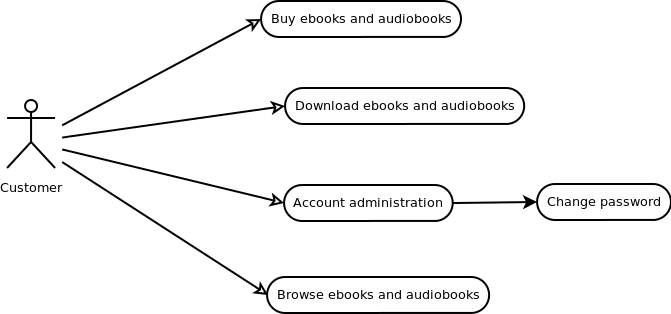
\includegraphics[scale=0.7]{Casemodel.png}
\caption{A use-case diagram describing the use cases of the Application.}
\label{casemodel}
\end{figure}

\subsubsection{Use-cases}

\begin{enumerate}
\item 
Title: Logging in\\
Entry condition: The user presses the log in button.\\
Main Success Scenario:\\
  Step 1: Then the user enters his/her username and password.\\
  Step 2: He/she then submits the information by pressing a button.\\
  Step 3: His/her books are now loaded to the application, as paths to the locally downloaded book.\\
Exit condition: The login is successful.\\
Extensions:\\
  Extension 2a: The user writes a wrong username and/or password.\\
  Extension 3a: There is no internet connection.\\
\item 
Title: Buying book\\
Entry Condition: The user presses the buy button, figure \ref{Book information}.\\
Main Success Scenario:\\
  Step 1: The user enters his/her credit card details.\\
  Step 2: He/she then submits the information by pressing a button.\\
  Step 3: The book is added to the users account.\\
Exit Condition: The book is successfully added to the user account, the book information side, figure \ref{Book information} will now show a download button instead of the purchase button.\\  
Extensions:\\
  Extension 2a: The user writes wrong card details.\\
  Extension 3a: There is no internet connection.\\
  Extension 3b: The transaction was denied.\\
\item 
Title: Search for a book\\
Entry Condition: The user presses the search bar.\\
Main Success Scenario:\\
  Step 1: A search query is written.\\
  Step 2: The query is committed.\\
  Step 3: The results are shown.\\
  Exit Condition: A book is chosen.\\
Extensions:\\
  Extension 3a: There is no internet connection.\\
  Extension 4a: The query returned no books.\\
\end{enumerate}
\subsubsection{Class diagram}
The class diagram shown in figure \ref{uml}, describes the outline of the solution-domain. This design is evolving with the project as new challenges arise. The current challenges that resulted in this solution domain are described in depth in section \ref{sec:Syssum}. The reason why it is changing is because we tried to be very specific about the attributes and functions from the beginning. Since then we have seen us forced to make changes.
\begin{figure}[H]
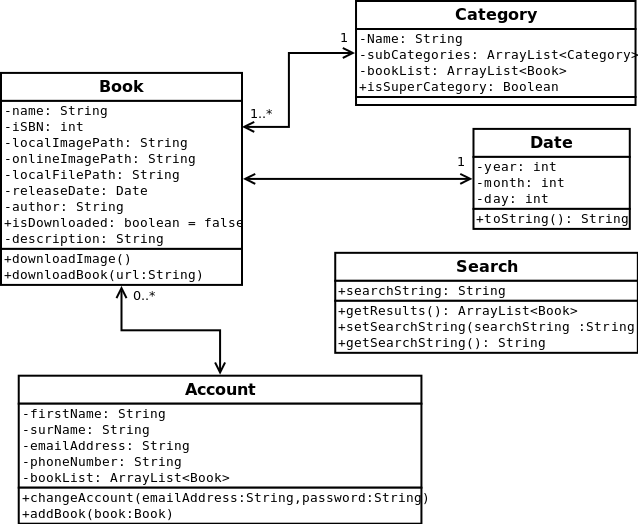
\includegraphics[scale=0.6]{uml.png}
\caption{A uml diagram over the Application}
\label{uml}
\end{figure}
\subsubsection{Sequence diagrams}

The sequence diagram shown in figure \ref{SeqDiaLogin} shows the chain of inner workings that is executed when the user tries to log in.
\begin{figure}[H]
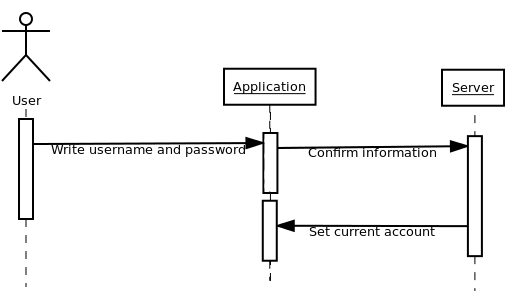
\includegraphics[scale=0.6]{SequenceDiagramLogin.png}
\caption{A sequence diagram for when a user logs in}
\label{SeqDiaLogin}
\end{figure}

The sequence diagram shown in figure \ref{SeqDiaBuyBook} shows the chain of inner workings that is executed when the user tries to buy a book.
\begin{figure}[H]
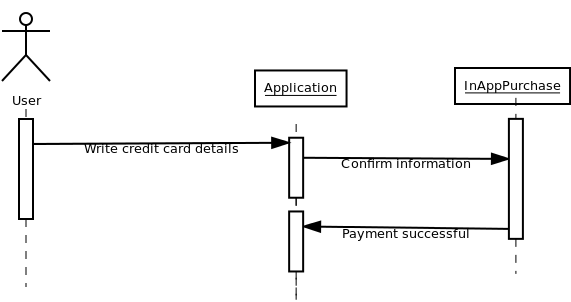
\includegraphics[scale=0.6]{SequenceDiagramBuyBook.png}
\caption{A sequence diagram for when a user buys a book}
\label{SeqDiaBuyBook}
\end{figure}

The sequence diagram shown in figure \ref{SeqDiaBookSearch} shows the chain inner workings that is executed when the user tries to search for books.
\begin{figure}[H]
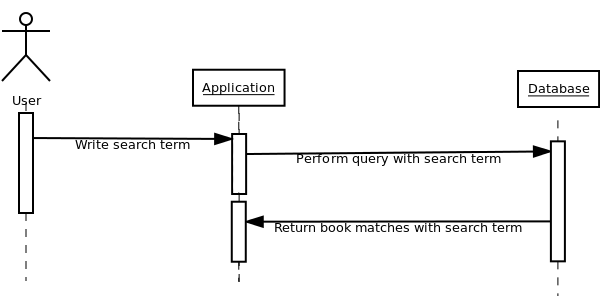
\includegraphics[scale=0.6]{SequenceDiagramBookSearch.png}
\caption{A sequence diagram for when a user searches for a book}
\label{SeqDiaBookSearch}
\end{figure}

\subsection{Systemdesign summary}
\label{sec:Syssum}
We have developed a prototype of the application that can be developed further on. If we choose to proceed with the project, we need to implement the following:\\

Database interaction through java:\\
The queries that the user makes regarding bought books and browsing for new books needs to be taken care of. The implementation of this depends on the WebAPI.\\
\\
A payment solution:\\
When a customer wants to buy a book, the system for handling this is needed. The Android SDK provides a tool for this, but it has yet to be implemented and fully understood.\\
\\
We also need a contract with a reader application as well as designing a login page when the application is launched.
\\\\
\newpage
\subsection{Program- and systemtest}

Our testing regime has involved emulating the lowest level API we are developing for and executing the application directly on our android smartphones, which uses the highest available API level. Furthermore, each incrementation has been loaded up in different screens sizes, to test that the layout scales correctly. However, this testing regime does not apply to our prototype as it is developed to showcase our progress. Finally, testing has involved black-box testing as described in the following subsection.

\subsubsection{Black-box testing}
We have been performing black-box testing when there was a 'screen' up and running, to examine the functionality of the applications. This was done by the group participants that had not been involved in the coding process of this particular screen so these people only knew what it was supposed to do and not how it did it. As of now, we have not encountered any major issues that required a reconsideration of the whole coding process. It has been minor bugs that were easily fixable without messing up how we had our system planned out.

\subsection{Userinterface and interaction design}
The external interfaces are here understood as the finished product GUI as it follows in Figure \ref{Front page},\ref{Book information},\ref{Categories} and \ref{Results}. The application GUI for the login page is yet to be designed.
\begin{SCfigure}
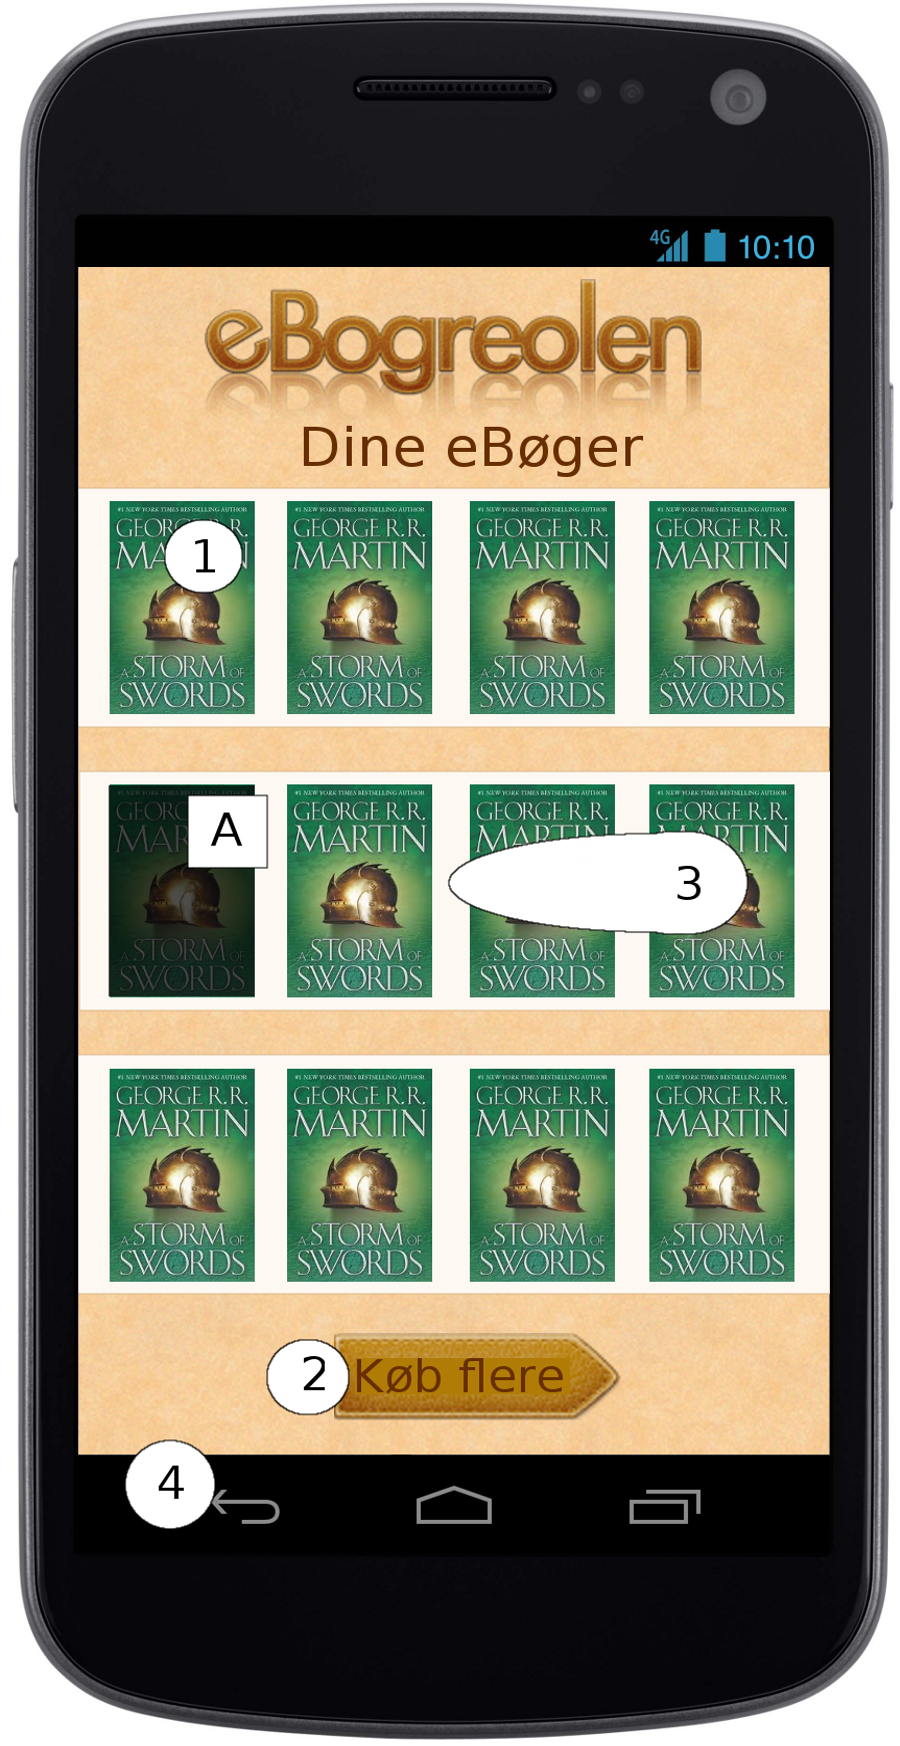
\includegraphics[scale=0.7]{gnexforside.png}
\caption{
\\
1. Open a page containing the information of a purchased book. This will lead to Figure \ref{Book information}.\\\\
2. Search/browse after more books to purchase. This will lead to Figure \ref{Categories}.\\\\
3. Swipe to the side to look at more of your books.\\\\
4. This button will always go one page back. If there are no more pages to go back to, the application will be closed.\\\\\\
A. This book is darkened, because the book has been purchased, but not downloaded.
}
\label{Front page}
\end{SCfigure}

\begin{SCfigure}
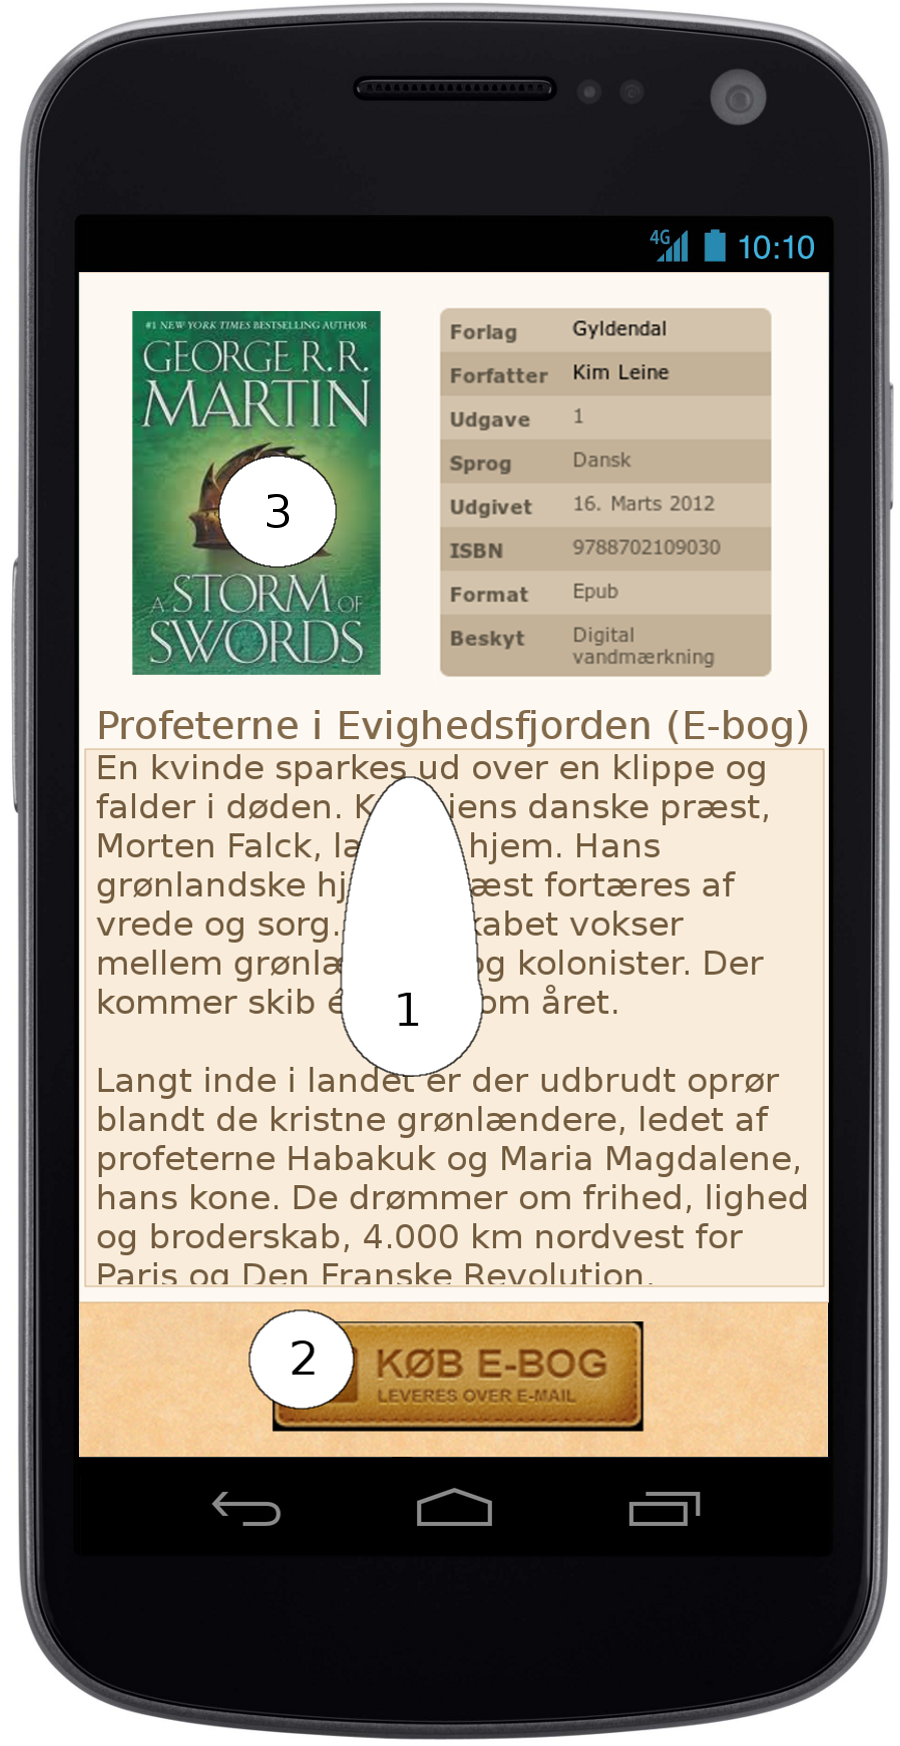
\includegraphics[scale=0.7]{gnexinfodownloadogkoeb.png}
\caption{
\\
1. Swipe up and down to read a description of the book.\\\\
2. This button can be a: Buy, Download, Read or Listen button, this depends on whether or not you own the material and/or if it is an audiobook or ebook.\\\\
3. Tapping the image enlarges it to a full screen view, tapping the image while enlarged will return to the displayed page.
}
\label{Book information}
\end{SCfigure}
\begin{SCfigure}
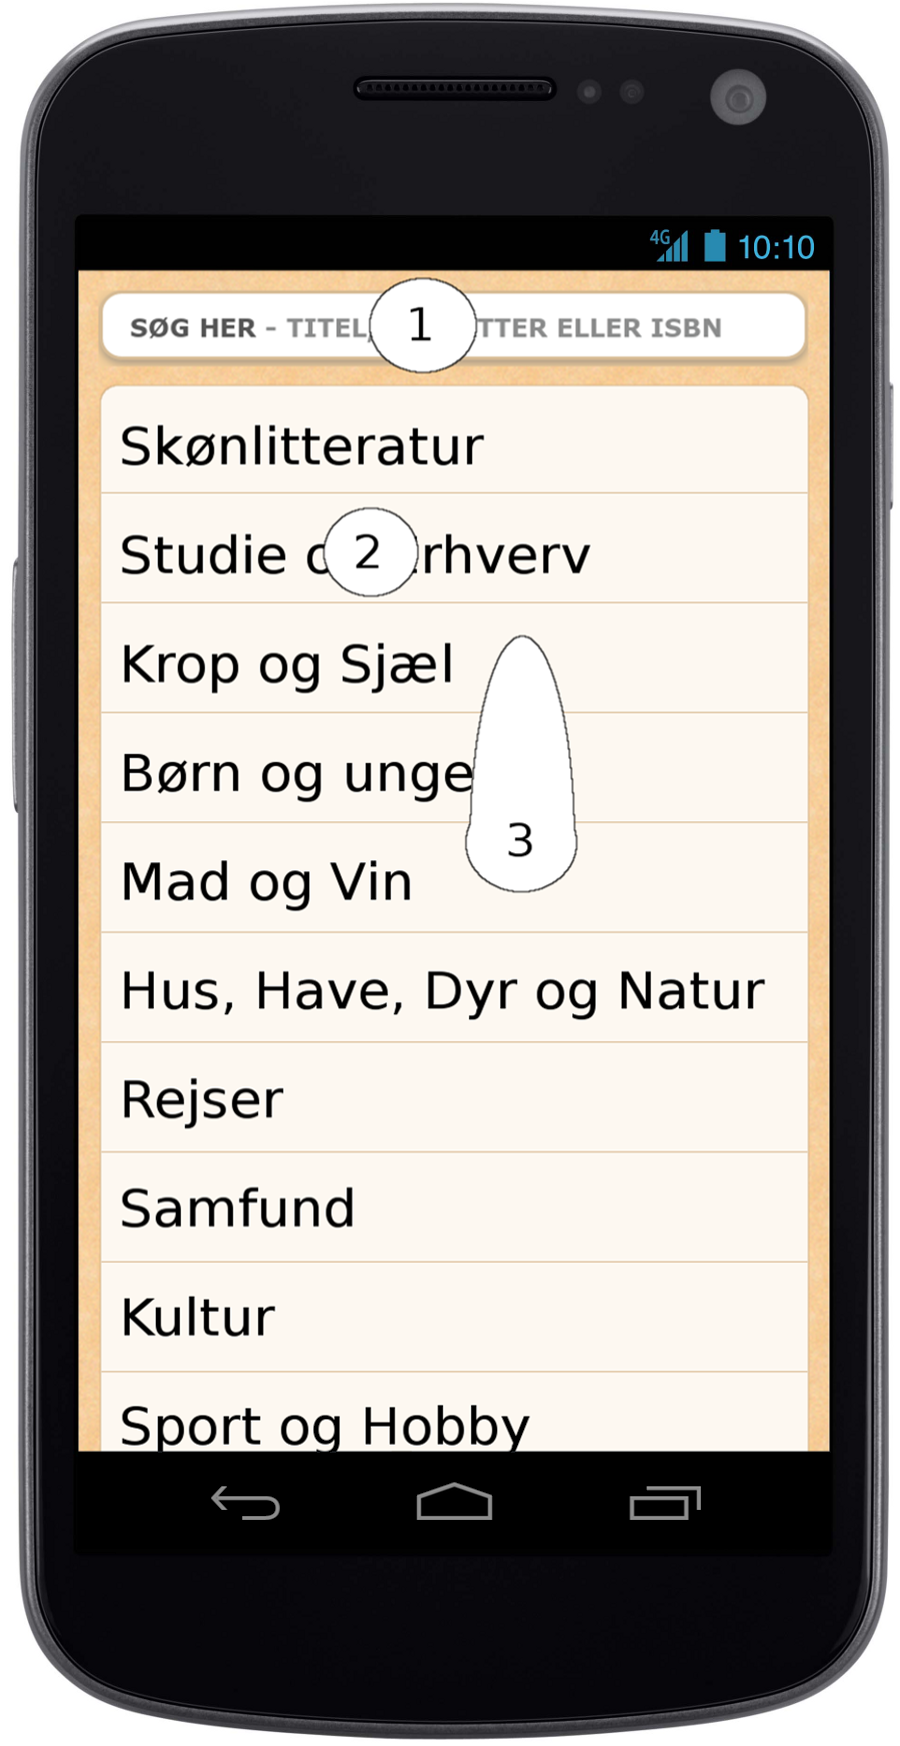
\includegraphics[scale=0.7]{gnexsoegeogbrowse.png}
\caption{
\\
1. This will access the search function, when a search is complete it will direct you to Figure \ref{Results}\\\\
2. This will open the category in this interface if it is a super category, and go to Figure \ref{Results} it is a sub category.\\\\
3. Swipe up and down to browse the categories.
}
\label{Categories}
\end{SCfigure}

\begin{SCfigure}
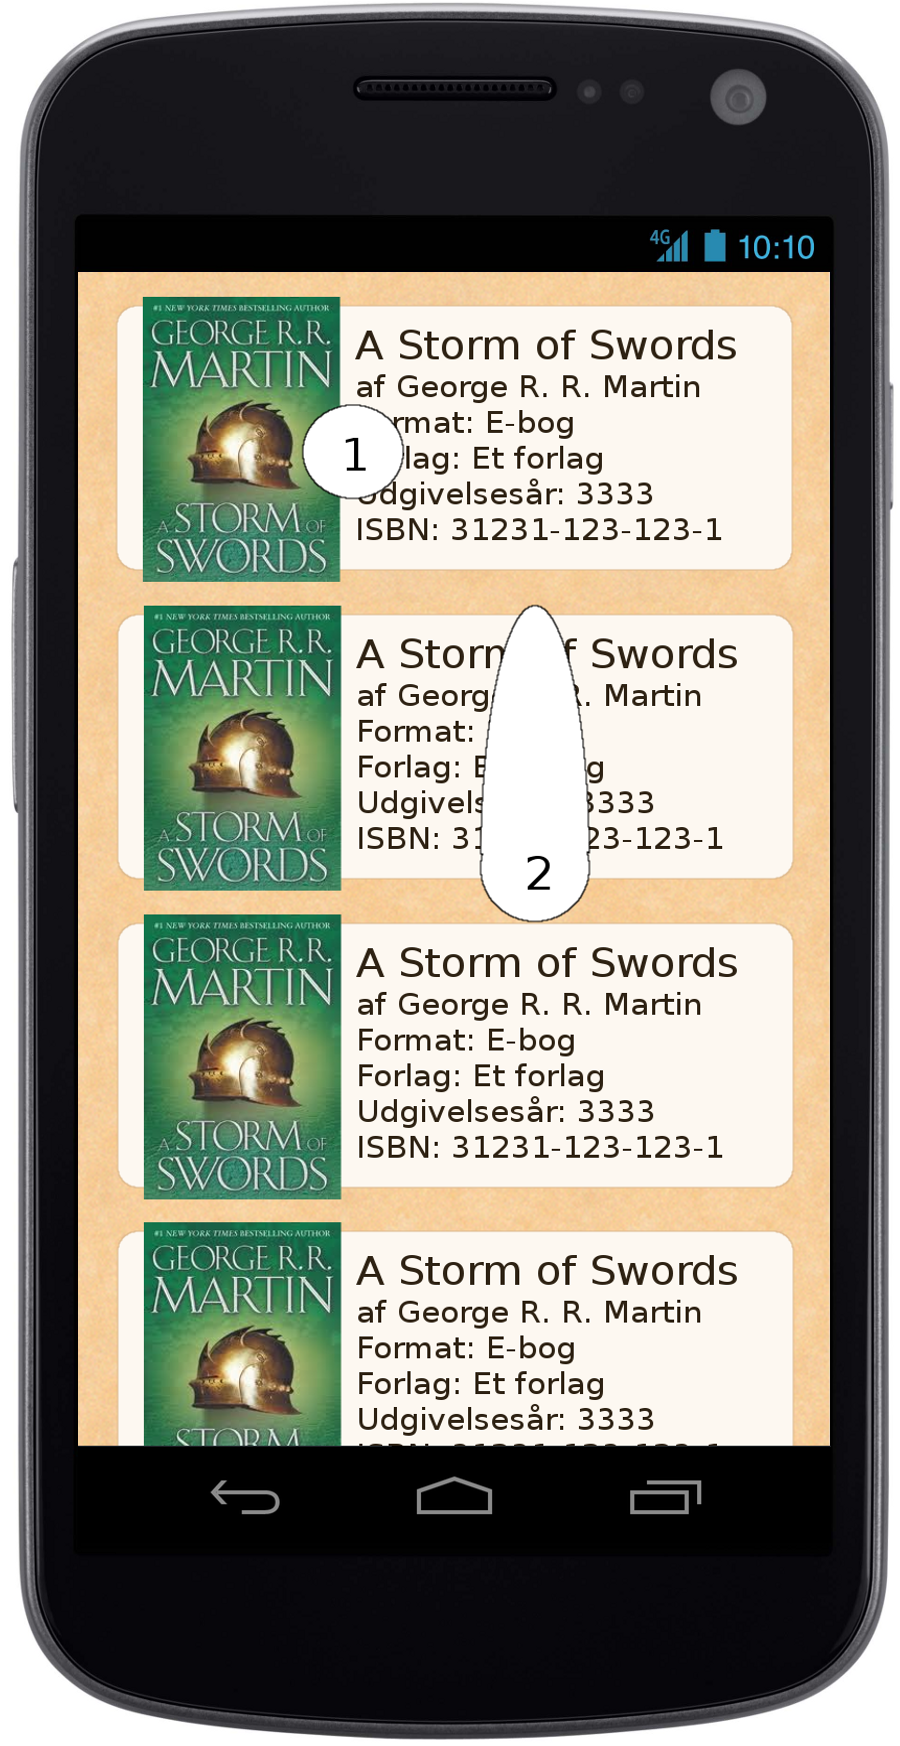
\includegraphics[scale=0.7]{gnexresultater.png}
\caption{
\\
1. This will take you to the information of the given book, this will lead to Figure \ref{Book information}.\\\\
2. Swipe up and down to browse the results.
}
\label{Results}
\end{SCfigure}

\subsubsection{Latest think-out-loud results}
The latest think-out-loud test was with a student who was asked to perform two tasks. Find a book called Storm of the Sword, then find the same book using a search, then purchase it and download the book to the device. The test was a pen and paper test using the activities figure  \ref{Front page}, \ref{Book information}, \ref{Categories} and \ref{Results}, without comments. The student was confused about the results page, \ref{Results}, but after explaining that this page would contain all the books fitting to the chosen category, he was appeased. The rest of the first task went smoothly. When asked to search for the book, the student identified the search bar fast on the categories
activity, \ref{Categories}. The student found it annoying that in order to purchase the book and download the book, he had to return to the same pages twice when being send back after doing the purchase.

\subsection{Link to YouTube-presentation}
We now have a interactive prototype, with some dummy functionality. A presentation of the prototype can be found here: http://www.youtube.com/watch?v=WopMZ3KZ7Zc.

\subsection{Selected work of the implementation}
Working with the scaling of the objects was very difficult and hard to understand. This was because XML used so-called 'weights' to determine how large object were compared to other objects in the same layout. Margins were also to be specified with weights. The advantage of this is it is easier to secure the layout is the same on all android smartphones. This made the implementation very obscure because the scaling would change if another object was added next to it. This also meant that there was no ideal way a screen would look. We had decided to make it look like figures \ref{Front page},\ref{Book information},\ref{Categories} and \ref{Results} that we had designed on an early stage, so we tried to match these as well as possible.\\
This caused a lot of trial and error because it was tough to picture how the scaling would look on the smartphone. We found no easier way to deal with this matter than the guesswork, so it would often take some time to complete.

\section{Project collaboration}
\subsection{Schematic overview}
\textbf{Beginning of the project:}\\
Our group met in the beginning of the course a couple of times to pick a client which had a project we all were motivated to work for. We ended up having a meeting with two clients where we decided to work with Android application development. This was our only face-to-face meeting with our client. However, we have communicated through e-mail and skype throughout the whole process.\\
We also had a scrum every week in the beginning where we got an overview of the project and instead of making sprints where we assigned tasks to each of us, we sat down and made the design for the application together. This was done as a mock-up using pen and paper and gave us a good understanding of the different screens and navigation between them which was a good starting point.\\
\\
\textbf{Midway in the project:}\\
In the middle of the course, we had not done any actual coding so we decided to try and plan some get-together days where we would sit down and code on the project.\\ 
Since none of us had any experience with development to android, we spend time learning it, but we felt it gave us an impression of how large the project was, which later turned out to be an underestimation. We discussed the requirements of the API with our client that their developer was working on, and when we could expect to receive it.\\
\\
\textbf{End of the project:}\\
In the last part of the course, we met several times during the last month for coding sessions. We worked on linking different activities, so as to make the application interactive. We finished most of the front-end, however, there were still some issues with the layout. We received the API from our client, but it was not implemented in the application due to limited time. However we made a prototype for the application with dummy data as seen in the YouTube presentation.\\
Since then we have talked about finishing the application when the course is finished.


\subsection{Relationship between parties}
All the planning was done by the group participants and we kept it within the group. We did have an e-mail correspondence running with our client, but it was mainly with focus on updating each other on how far we were in the process seen in the bigger picture. We did not update each other on smaller tasks only on critical things.\\
Because of this, it was hard to grasp the size of the project because there sometimes went weeks between updates which also meant, that when the API from our client came later than expected, we realised we misjudged the time needed to finish the application.\\

\subsection{Collaboration in the group}
Our group has worked very well with few conflicts of interest. We all knew each other before the beginning of the project so we get along very well.\\
All our decision is based on a mutual agreement. Since we had different strengths and weaknesses, our group was good to help each other and make sure everyone understood the problem fully if something occurred. That way everyone was not very far behind others and as a result the work was distributed as well as it could across all of the group members.\\
Furthermore, we created a 'game' to keep motivations high, making sure it was just for fun and not to be taken completely serious. See \ref{game} for more information on this.

\subsection{Strength and weaknesses in the process}
Our group was very effective to get a project running using an advertisement as well as calling people asking if they needed an android application for their business. We had already established to develop in android for this project. We quickly arranged a couple of meetings and, upon picking a client, was fast to design the application as a mock-up in pen and paper which made the foundations of the final product as well. The choice of programming language and version control used in the project was the right choice since it was all something we had experience in or had heard of.\\
The mock-up worked much better than expected, since it allowed us to see how the application would be most intuitive and it was easy to make changes to if we found errors in the design. This is also mentioned in "Ehn, P. and Kyng, M. (1991), Cardboard computers: Mocking-it-up or hands-on the future."\\
However, our planning could have been better. Even though we were very effective in the beginning, we calmed down because we underestimated the amount of work. This could be because we had not tried to make a prototype to get a feeling on how far we were in the process.

\subsection{Improvements}
We should have been faster to make sprints instead of waiting for the API to come. We tried to assign tasks to the members when we got it, but it was unsuccessful since android development proved harder than it seemed and required more time than we had set aside for it. A better planning with scrums more often could have prevented that.\\
Setting up git and github faster could also immensely have improved our working process. It was up and running very late and we almost only used to put the pieces together to create the prototype.

\newpage
\section{Review: Building Products as Innovation Experiment Systems by Jan Bosch}
\subsection{Article summary}
The article discusses the procedure of releasing a product while increasing customer interest and consequently, improve revenue. It examines the differences between traditional software development and "innovation experiment system" (IES).\\
The article states there is a growth in SaaS (Software-as-a-Service) because the commitment from the customer is not as high and that both software in connected embedded systems and SaaS has frequent updates instead of licensed software where the release is supposed to be usable by the customer in a longer period of time and the cost is larger.\\
This has led to the customer being accustomed to frequent updates and as such, ideas is needed to update or release the right things to satisfy as many customers as possible. By collecting feedback from customers it is easier to see what ideas is worth researching and developing in.\\
There exists different ways of collecting the feedback from customers depending on what type of product is to be released, e.g new features to a product, a new product or optimization. It also depends on what stage the implementation is in, e.g. pre-development, non-commercial deployment, commercial deployment. The article discusses different strategies to evaluate what ideas are best and make sure research and development is in the ideas which will have the largest amount of customer interest and, in the end, the highest revenue, depending on what kind of product it is.\\
Conclusively, the article says that a new development model is different from the traditional model. There needs to be frequent updates, customer and their feedback plays a big part in the whole development process and the development process is about testing many different ideas.

\subsection{Discussion of main points}
\textbf{Licensed software is not as successful anymore}\\
I agree that other models, such as the freemium model where you have access to basic features for free but can choose to pay a small fee to unlock the all the features is becoming more and more successful, as it is especially seen in applications to smartphones. Often the fees are very small and so the customers do not see a reason to buy it if they liked the free version. \\
For applications, it is almost a must to have a free version, because otherwise customers would be quick to discard it in the first place and thus the interest would be very low. If it requires an investment, it scares potential customers away. When it is free, the customer can freely examine the product without feeling any commitment and choose to buy the full version if it is something worth paying for.\\
\\
\textbf{Software is more successful with frequent updates}\\
I agree completely with this. Drawing from own experience, a product with no running development feels like it is a dead product. Where knowing there will be new content is comforting and feels like there is put more work into it. Furthermore, you are secured that the product you pay for does not go out of date. \\
\\
\textbf{Testing and feedback on all stages of development}\\
This is very relevant, since it allows the developers to examine what things customers want to see working, so called "costumer pain". In the end, it is developed for costumers and naturally it would make sense to make these parts functional, redone or optimized as the first thing to avoid situations where half the design has to be discarded.\\
We did not make enough tests. Our testing only consisted of testing it ourselves. We got a thumbs up from eBogreolen about our design when we released it to them, but we never questioned if that was what the customers would actually like to see in such an application. With the final product, we can not be sure we have developed the right thing so to say. Maybe we left out features that would really have appealed to many costumers or we implemented some features that does not appeal to as many costumers as it could have. Constant testing on potential costumers, or simply people not associated with the project, would have given a heads up if we were heading down the wrong path.\\
In our case we wanted to introduce a new product, but it was already a prototype when we started to test it on persons. Had we been testing while we only had designed the mock-up, we could have avoided potential faults that might have to be redone later. In this case, it is not very costly, but had it been a larger project that had required a large investment, it could have been a serious set back if the product did not live up to the costumers' expectations and something in the design had to be reworked.
 
\newpage 
\section{Appendix}
\subsection{Motivation game}
\label{game}
We have developed scoreboard as a motivational tool, which entitles the person in lead to small benefits (bragging rights, beers etc.). This has benefited the group immensely as we all thrive in a competitive environment. Our scoreboard uses 'experience' points, gained through working with the project and completing tasks associated with our sprint backlog. These experience points are distributed to the group participants by a point generator, found here: \url{http://www.VixQIT/XP/XP.php}, that generates a random amount of points in a certain range around x. Tasks are worth points equal to the hours of work estimated during our scrum and these translates into points that provides the range from your random gain of experience. The experience needed to level up increases each time following the Fibonacci sequence.\\

\end{document}